\chapter{Bearbeitung der Aufgaben}
\section{Geschichteter Plattenkondensator}

Möchte man numerisch die Kapazität eines Plattenkondensators mit quer geschichtetem Dielektrikum mit linear steigender relativer Permittivität bestimmen, kann man den linearen Verlauf über mehrere Schichten mit jeweils konstanter Permittivität approximieren. Wie bei numerischen Verfahren üblich wird die Approximation besser, je kleiner man die einzelnen Schichten wählt.\\
Die Funktion \texttt{femmcapacity.m} bekommt als Parameter den Abstand $h$ zwischen den beiden Platten des Kondensators, die Kantenlänge $a$ der quadratischen Platten, $\epsilon_{r1}$, $\epsilon_{r2}$ und die Anzahl $N$ an Schichten übergeben und erzeugt daraus einen Plot für den Potentialverlauf im Kondensator und berechnet die Kapazität der Anordnung. Die relative Permittiviät variert hierbei linear zwischen $\epsilon_{r1} $ am linken Rand und $\epsilon_{r2}$ am rechten Rand. Im Folgenden werden als Abstand zwischen den Platten und als Kantenlänge 30cm angenommen. Wählt man 9 Schichten, $\epsilon_{r1} = 1$ und $\epsilon_{r2} = 2$  erhält man den in Abbildung \ref{fig:N9} zu sehenden Potentialverlauf und eine Kapazität $ C_1 = \num{3,793}\si{\pico\farad}$.

\begin{figure}[h]
	\begin{subfigure}[c]{0.3\textwidth}
		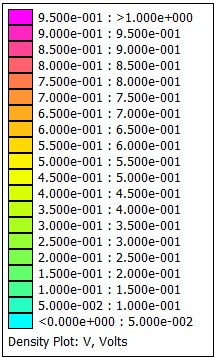
\includegraphics[width=\textwidth]{data/KondensatorN9_Legende}
		\caption{Skala}
		\label{fig:Skala1}
	\end{subfigure}
	\begin{subfigure}[c]{0.6\textwidth}
		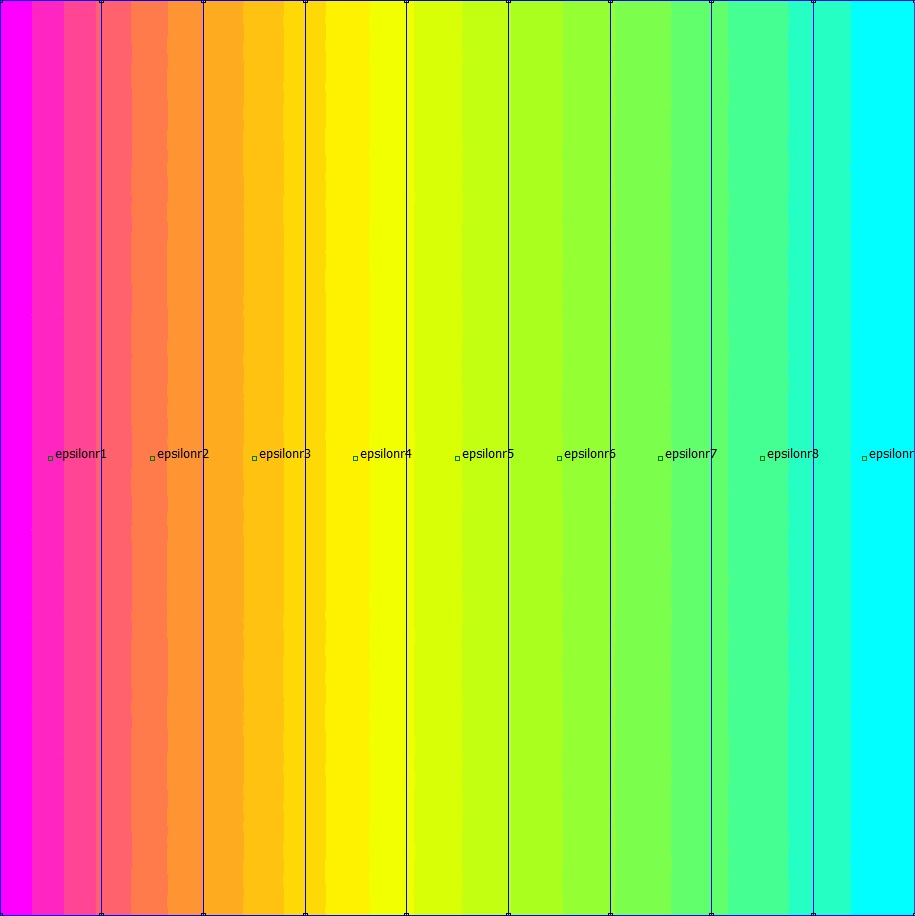
\includegraphics[width=\textwidth]{data/KondensatorN9}
		\caption{Potentialverlauf im Plattenkondensator mit 9 Schichten}
		\label{fig:N9}
	\end{subfigure}
	\caption{Potentialverlauf im Plattenkondensator mit 9 Schichten}
\end{figure}

Wiederholt man die Simulation für $N = 1,2,3,...,20$ Schichten und lässt sich in einem Konvergenz-Plot (Abbildung \ref{fig:semilogy}) die Kapazität in Abhängigkeit der Schichtenanzahl anzeigen, erkennt man, dass schon nach $N=3$ Schichten die Kapazität annähernd exakt bestimmt wird und weiter Verfeinerungen nur noch marginale Verbesserungen erzielen. 

\begin{figure}[tpbh]
	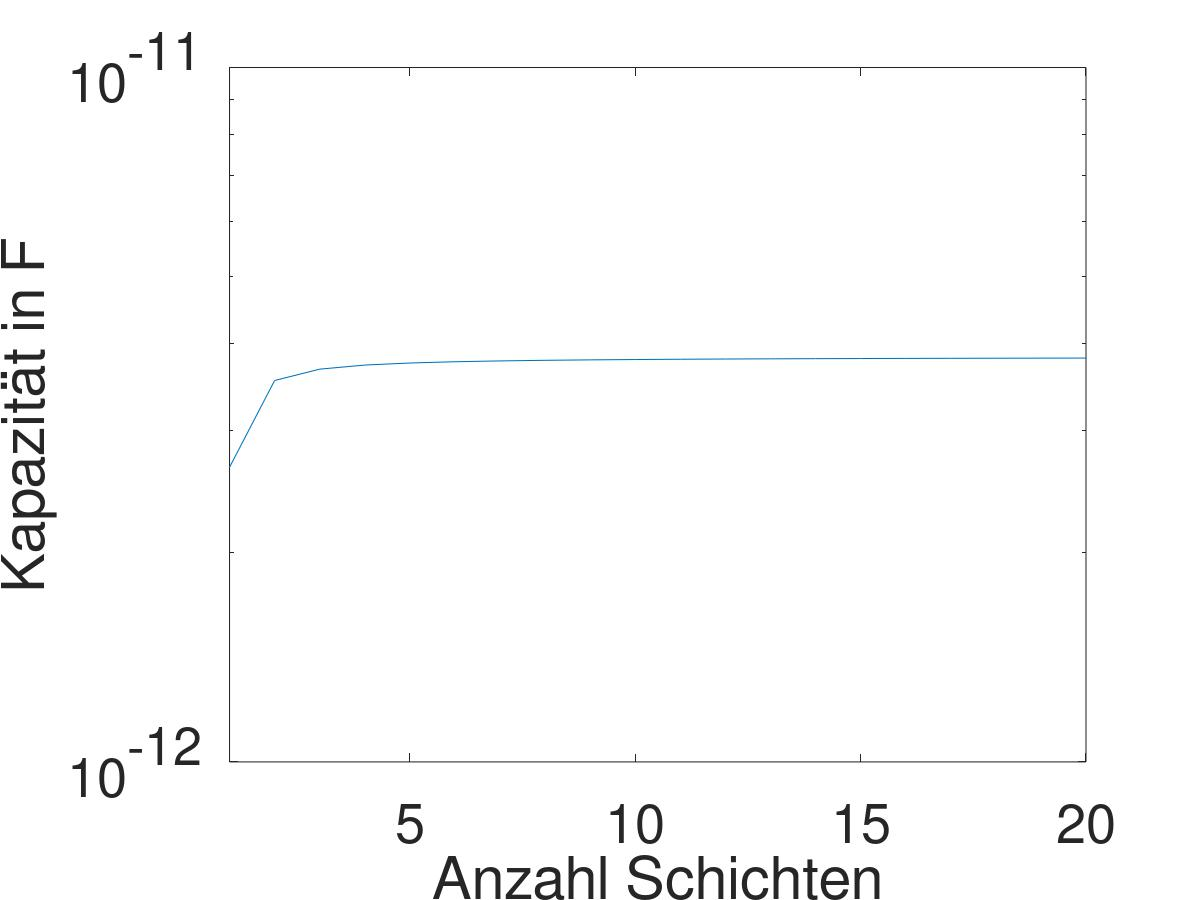
\includegraphics[width=0.6\textwidth]{data/Kapazitaet}
	\caption{Änderung der Kapazität mit steigender Anzahl an Schichten im Plattenkondensator}
	\label{fig:semilogy}
\end{figure}


Die Option 'Vector Plot' in FEMM ist nützlich um den Verlauf des elektrischen Feldes besser darzustellen. Die Richtung der Pfeile zeigt an in welche Richtung das Feld an dieser Stelle zeigt und die Länge der Pfeile deutet die Stärke an dieser Stelle an.\\
In Abbildung \ref{fig:N1_EFeld} sieht man den Plot für den homogenen Plattenkondensator und in Abbildung \ref{fig:N9_EFeld} für den geschichteten Fall. Vergleicht man die beiden Abbildungen fällt auf, dass das elektrische Feld im homogenen Plattenkondensator ebenfalls homogen verteilt ist. Beim geschichteten Plattenkondensator hingegen ist das elektrische Feld deutlich stärker auf der Seite mit der geringeren relativen Permittivität und nimmt dann immer weiter ab je höher die relative Permittivität ist.

\begin{figure}[h]
	\begin{subfigure}[c]{0.2\textwidth}
		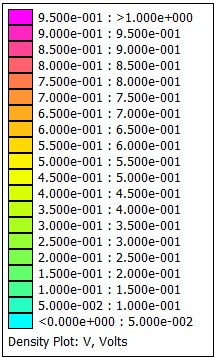
\includegraphics[width=\textwidth]{data/KondensatorN9_Legende}
		\caption{Skala}
		\label{fig:Skala2}
	\end{subfigure}
	\begin{subfigure}[c]{0.35\textwidth}
		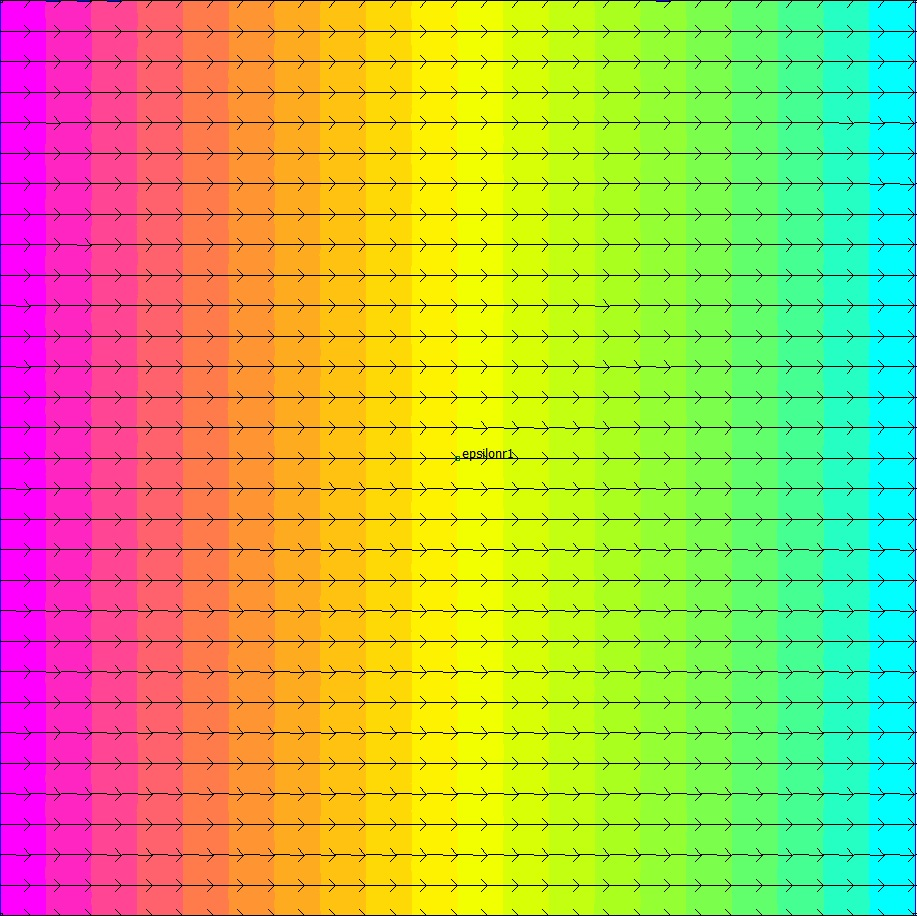
\includegraphics[width=\textwidth]{data/KondensatorN1_EFeld}
		\caption{Potentialverlauf und elektrische Feldstärke im homogenen Plattenkondensator}
		\label{fig:N1_EFeld}
	\end{subfigure}
	\begin{subfigure}[c]{0.35\textwidth}
		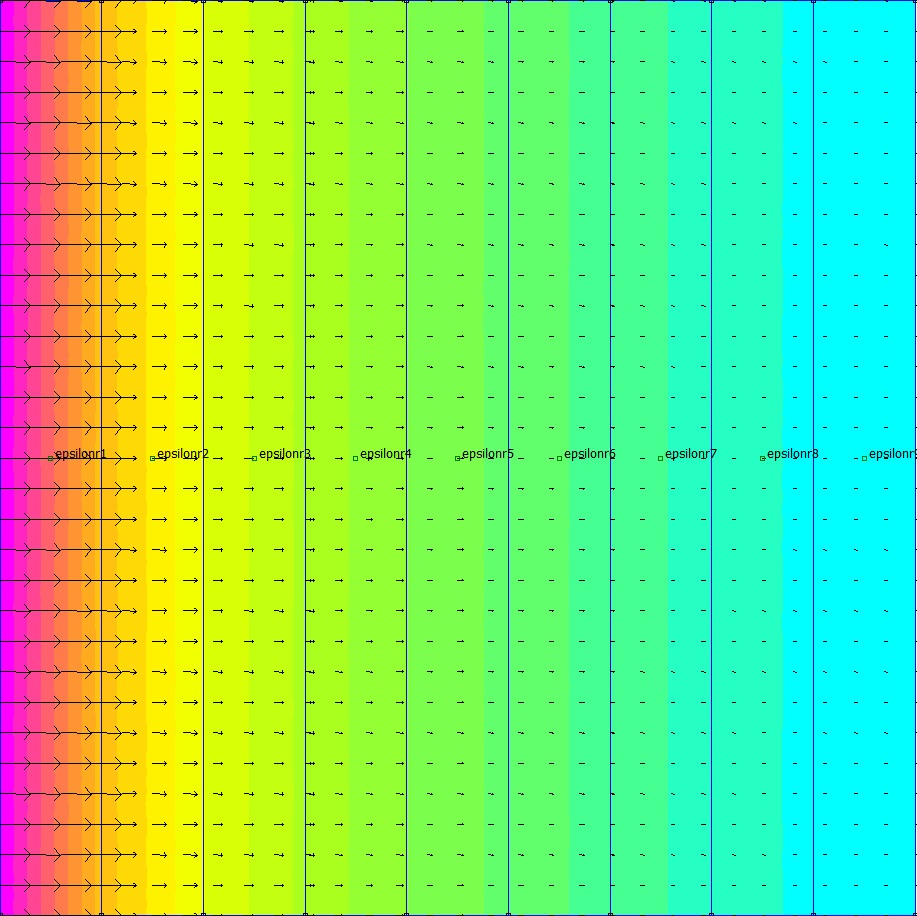
\includegraphics[width=\textwidth]{data/KondensatorN9_EFeld}
		\caption{Potentialverlauf und elektrische Feldstärke im Plattenkondensator mit 9 Schichten}
		\label{fig:N9_EFeld}
\end{subfigure}
	\caption{Potentialverlauf und elektrische Feldstärke im homogenen und im geschichteten Plattenkondensator}
\end{figure}

Bestimmt man die Kapazität für $\epsilon_{r1} = 1$ und $\epsilon_{r2} = 10$ und $N = 9$ und vergleicht diese mit der vorher bestimmten Kapazität $C_1$ stellt man fest, dass durch eine höhere relative Permittivität auch die Kapazität von $\SI{3,793}{\pico\farad}$ auf $\SI{8,916}{\pico\farad}$ steigt.

